\graphicspath{{chapters/greco/images/level7/}}
\subsection{GRECO Level 7: Final Level}

\label{subsec:pegleg_reco}
\subsubsection{Reconstruction using PegLeg}
The existing reconstructions up to this point use either analytic or simplified likelihood reconstructions to estimate particle parameters.
The position of the first hit and the finite muon reconstruction from FiniteReco provide straightforward separation power between atmospheric muons and neutrino events, but are designed to be computationally inexpensive instead of precise.
At final level, these estimates are refined using a novel reconstruction method developed specifically for low-energy and oscillation searches with DeepCore.

The \textbf{PegLeg} reconstruction, developed by Martin Leuermann based, in part, on earlier work by Matt Dunkmann, is a low-energy reconstruction that uses a hybrid cascade+muon hypothesis.
The reconstruction returns a total of eight parameters: the position ($x_R$, $y_R$, $z_R$), time ($t_{R}$), direction ($\theta$, $\phi$), total energy ($E_{R}$) and track length ($L_{R}$). 
The algorithm requires both seeds for each of the particle parameters, a collection of hits over which to run, and a set of splines fit to an ice model.

For each particle hypothesis, the event is broken into steps in time based on the timing of the observed hits in the event.
At each time step, the expected charge at each DOM is calculated based on the energy and position of the particle emission scaled using the ice model splines.
The charge expectation is evaluated for all DOMs, regardless of whether a hit is observed or not.
The total likelihood of the hypothesis is then the product of the likelihoods at each DOM.

The likelihood space itself typically possesses multiple local minima due to the small number of hits.
The fit is performed using the MultiNest minimizer package \findref{multinest} in order to handle the complex likelihood space.

Given the large dimensionality of the space, significant computational power is required for the fit.
Various steps are used in order to reduce the resource requirements.
Track lengths are limited to integer values that depend on parameters used to produce the spline tables. 
While this requirement is lifted in newer versions of the software, that change has not yet propagated to the current GRECO events.
In addition, only DOMs within 150 meters of the current particle position are evaluated to find the expected charge.
All other DOMs are assumed to have an expected charge consistent with noise rates.
This assumption allows the minimizer to avoid costly calculations of expected charge for distant DOMs at the expense of higher energy event resolutions. \findref{martin's thesis}

In early versions of the PegLeg fit, the charge of individual pulses is used directly in the likelihood calculations \findref{millipede paper}.
Following the discoveries discussed in \ref{subsubsec:charge_templates}, however, the handling of the charge was changed \findref{martin's thesis}.
In the version of PegLeg used in the final version of this analysis, a deadtime window of 45 nanoseconds is introduced for each DOM directly following a pulse. 
During this window, the DOM may not contribute any further information to the fit, instead simply being labeled as "active".
This changes the reconstruction likelihood from being charge-based to being hit-based.
Using this modification, disagreements between the data and simulated pulses may be minimized.

Each event takes approximately 15 minutes on average to converge in the reconstruction.
There also exists a significant tail to the reconstruction time, sometimes extending to multiple hours for a single event.
With a large expected sample of events, the reconstruction time is the most computationally intensive part of the event selection

\label{subsubsec:pegleg_containment}
\subsubsection{Containment with PegLeg}
With a more refined reconstruction, additional constraints on the containment of the starting verticies are possible.
Similar to the work done with FiniteReco at L6, the $Z_R$ and $\rho_R$ recieve cuts in two dimensions as shown in \ref{fig:pegleg_zVsRho}.
Once again, events at the top of and near the edge of DeepCore are more likely to be muons.
An additional cut is applied at the bottom of the detector in order to limit the effect of observed discrepancies data and Monte Carlo.
Removing these events results in a 75\% reduction of the atmospheric muon background at a cost of approximately 10\% of the overall neutrino rate.

\begin{center}
\begin{table}
\begin{tabular}{cc}
    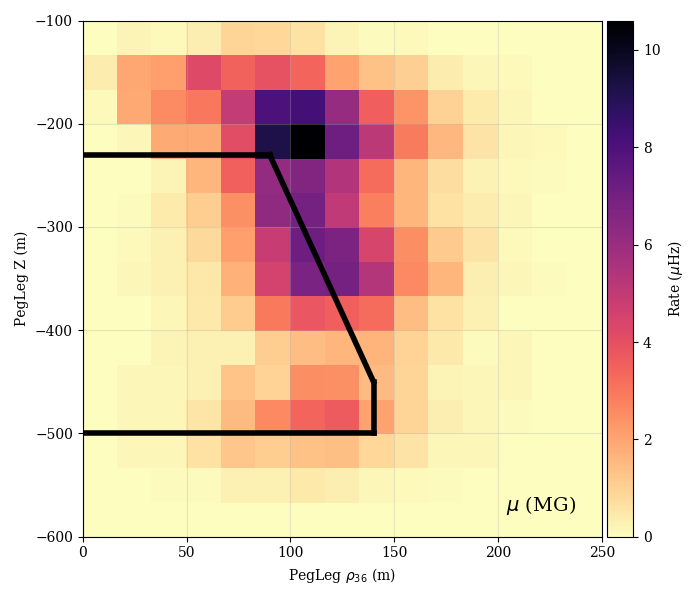
\includegraphics[width=0.45\linewidth]{pegleg_z_rho_muongun.png} &  
    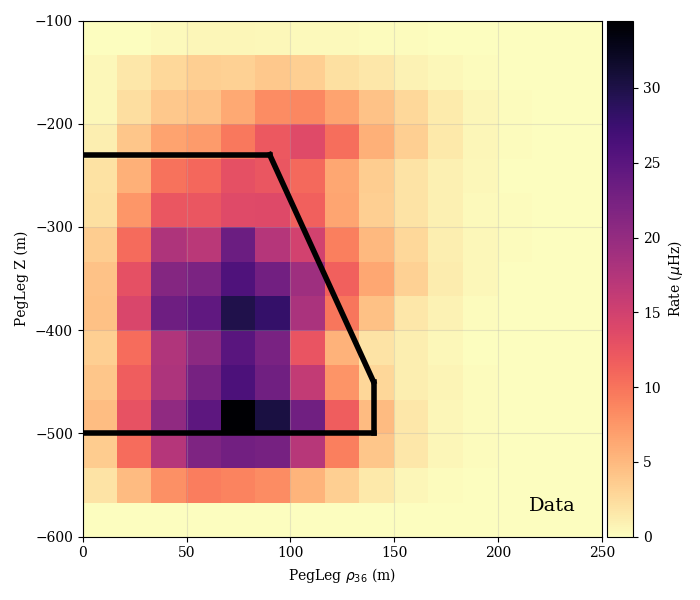
\includegraphics[width=0.45\linewidth]{pegleg_z_rho_data.png} \\  

    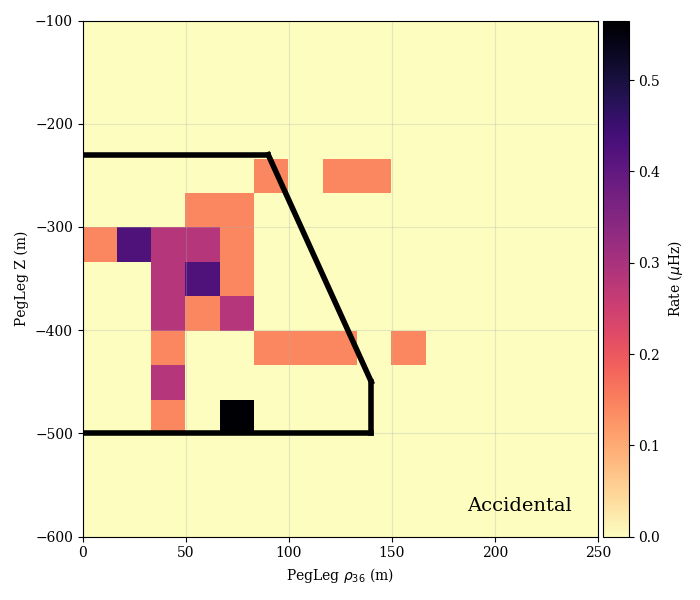
\includegraphics[width=0.45\linewidth]{pegleg_z_rho_noise.png} &  
    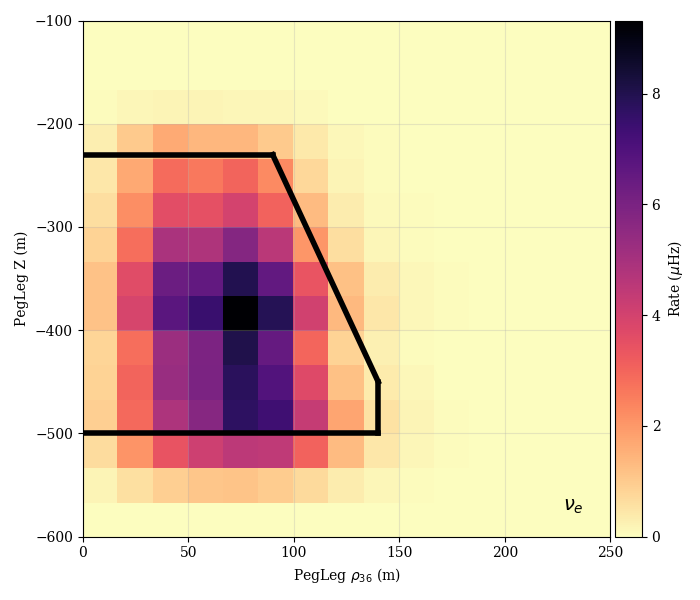
\includegraphics[width=0.45\linewidth]{pegleg_z_rho_genie_nue.png} \\  

    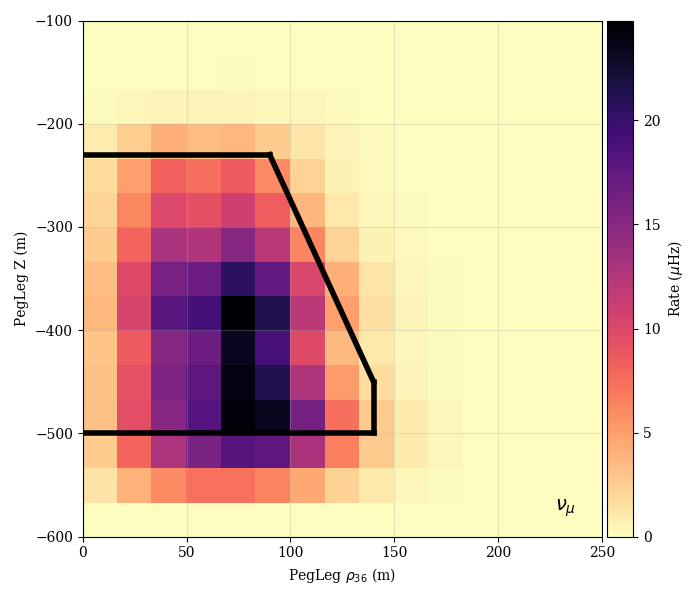
\includegraphics[width=0.45\linewidth]{pegleg_z_rho_genie_numu.png} &  
    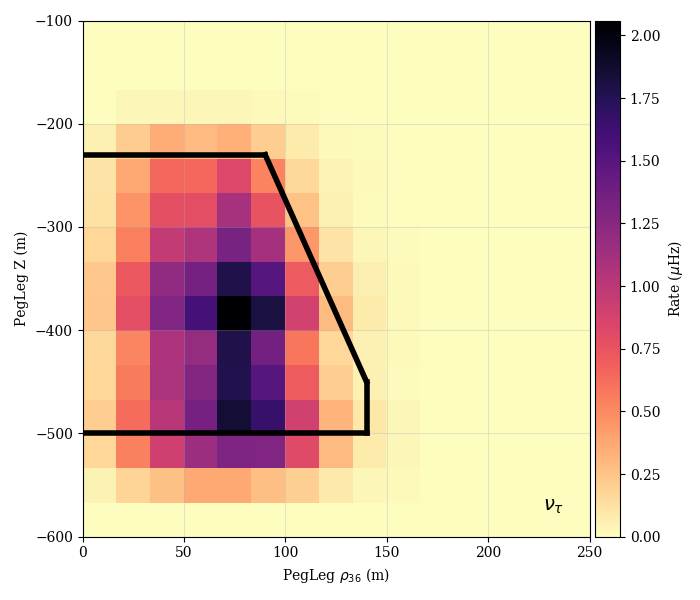
\includegraphics[width=0.45\linewidth]{pegleg_z_rho_genie_nutau.png} \\ 
\end{tabular}
\label{fig:pegleg_zVsRho}
\caption{The PegLeg L7 containment cut for each of the channels. The cut itself is shown with the black line. Note that the atmospheric muons are here represented by the higher-statistics MuonGun sample.}
\end{table}
\end{center}

\label{subsubsec:other_l7_cuts}
\subsubsection{Other Cuts at L7}
In the course of further work on the event selection, a number of issues previously-unknown were discovered.
The most important of these, discussed further in \ref{subsubsec:flaring_doms}, is the discovery of flaring DOMs, where a DOM spontaneously emits light.
Because the light is emitted from the DOM itself, these events are characterized by high light yield on a single DOM relative to the rest of the event.
These events were first discovered with the GRECO sample and are under further investigation within the IceCube collaboration.
Two DOMs are known to emit light in this way at a rate of approximately once per day, although more are under investigation as of the time of this writing. 

The two known DOMs are removed from the reconstruction pending further investigation. 
In addition, any event event with a single DOM observing more than 80\% of the total charge is removed to remove events with this characteristic signature.

Cuts are also applied to the average reconstructed energy per hit DOM (\ref{fig:gev_per_nch}) and the scatter in the timing distribution of hits (\ref{fig:t_rms}).
The former is expected to yields high values for events dominated by flaring DOMs or events where a particle interaction occurs very close to the face of a DOM.
The distribution also shows some disagreement at low values, however.
The reason for this is likely related to the issues discovered in \ref{subsubsec:charge_templates}, although this disagreement has not been investigated further.
A cut removing events with more than 3 GeV/DOM is applied only to events with fewer than 14 hits, limiting the impact on the neutrino signal events.

The scatter in the hit times shows very good agreement between data and simulation and is useful as a proxy for the overall scattering of the event.
The cut, which removes events with a root-mean-square hit time of 600 nanoseconds, is also only applied for events with fewer than 14 hits.
This limits the loss of neutrino events while removing a fraction of the remaining accidental triggers.

\begin{center}
\begin{table}
\begin{tabular}{cc}
	\label{fig:gev_per_nch} 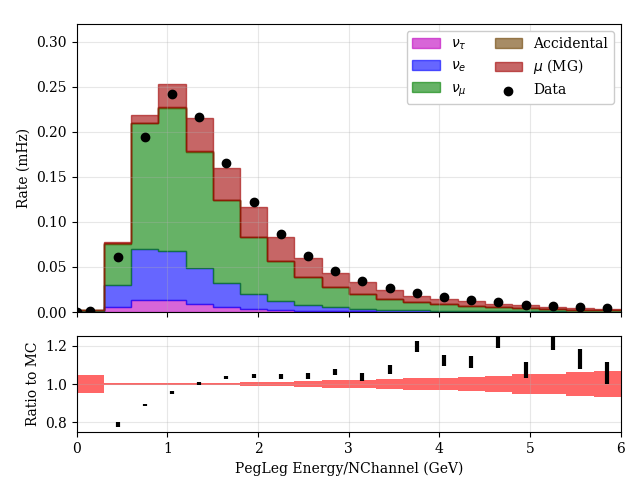
\includegraphics[width=0.45\linewidth]{L7_GeV_per_channel.png} &
	\label{fig:t_rms} 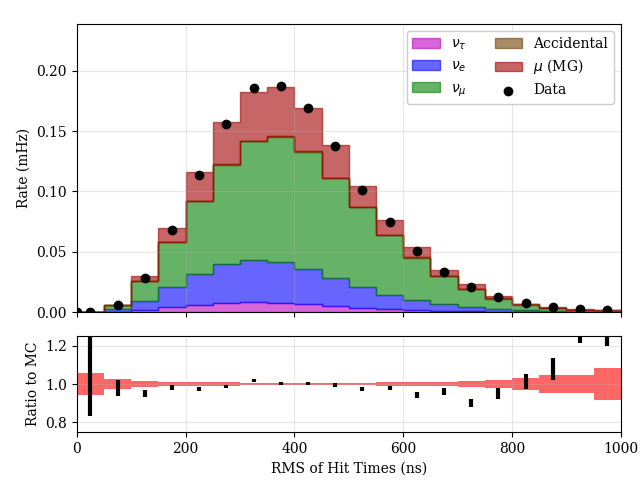
\includegraphics[width=0.45\linewidth]{L7_t_rms.png} \\
\end{tabular}
\caption{The final two cuts applied to the sample prior to the analysis binning. All events are included here, although each cut is only applied to events with fewer than 14 hit DOMs. Note that the total simulation rate is scaled downward by 20\% to approximately match the rate of the data events.}
\end{table}
\end{center}
